\documentclass[answers]{exam}


\RequirePackage{amssymb, amsfonts, amsmath, setspace, graphicx}
\usepackage[margin=1in]{geometry}


% Here's where you edit the Class, Exam, Date, etc.
\newcommand{\classnum}{MAT 2000}
\newcommand{\classname}{Introduction to Statistics}
\newcommand{\examname}{Quiz: Section 2.1}
\newcommand{\school}{Grace College}

%Shortcuts:
\newcommand{\nn}{\mathbf{N}}
\newcommand{\zz}{\mathbf{Z}}
\newcommand{\qq}{\mathbf{Q}}
\newcommand{\rr}{\mathbf{R}}
\newcommand{\cc}{\mathbf{C}}

% For an exam, single spacing is most appropriate
\singlespacing
% \onehalfspacing
% \doublespacing

% For an exam, we generally want to turn off paragraph indentation
\parindent 0ex

\begin{document}
	
	\pagestyle{head}
	\firstpageheader{}{}{}
	\runningheader{\classnum}{\examname\ - Page \thepage\ of \numpages}{\school}
	\runningheadrule
	
	\begin{flushright}
		\begin{tabular}{p{2.8in} r l}
			\textbf{\examname} & \textbf{Name (Print):} & \makebox[2in]{\hrulefill}\\
			\textbf{\classnum} &&\\
			\textbf{\classname} &&\\
			\textbf{\school}
			%\textbf{Time Limit: \timelimit} & Teaching Assistant & \makebox[2in]{\hrulefill}
		\end{tabular}\\
	\end{flushright}
	\rule[1ex]{\textwidth}{.1pt}
	
	\begin{questions}
		\uplevel{Do red uniform wearers tend to win more often than those wearing blue uniforms in tae-kwon-do matches where competitors are randomly assigned to wear either a red or blue uniform? In a sample of 80 tae-kwon-do matches, there were 45 matches where the red uniform wearer won.
			
		Refer to this scenario for questions \ref{twd1}-\ref{twd4}}
		
		\question \label{twd1} What is the parameter of interest for this study?
		
		\begin{choices}
			\correctchoice The long-run proportion of tae-kwon-do matches in which the red uniform wearer wins
			\choice The proportion of matches in which the red uniform wearer wins in a sample of 80 tae-kwon-do matches
			\choice Whether the red uniform wearer wins a match
			\choice 0.50
		\end{choices}
		
		\question \label{twd2} What is the statistic for this study?
		
		\begin{choices}
			\choice The long-run proportion of tae-kwon-do matches in which the red uniform wearer wins
			\correctchoice The proportion of matches in which the red uniform wearer wins in a sample of 80 tae-kwon-do matches
			\choice Whether the red uniform wearer wins a match
			\choice 0.50
		\end{choices}
		
		\question \label{twd3} Given below is the simulated distribution of the number of "red wins" that could happen by chance alone in a sample of 80 matches. Based on this simulation, is the observed result statistically significant?
		\begin{center}
			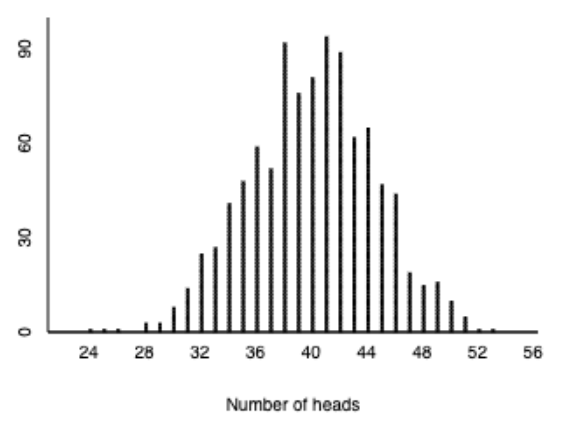
\includegraphics[width = 0.5 \linewidth]{sim1.png}
		\end{center}
		\begin{choices}
			\choice Yes, since 45 is larger than 40.
			\choice  Yes, since the height of the dotplot above 45 is smaller than the height of the dotplot above 40.
			\correctchoice  No, since 45 is a fairly typical outcome if the color of the winner's uniform was determined by chance alone.
			\choice  No, since an observed value greater than 45 could just be by random chance.
		\end{choices}
		
		\question \label{twd4} What can be concluded from the results of this study? Select the option that does NOT apply.
		\begin{choices}
			\choice The results of this study are something that could easily have happened if the color of the winner's uniform was determined by chance alone.
			\choice Convincing evidence does not exist against the "by-chance-alone" model.
			\correctchoice The results of this study prove that the color of the winner's uniform was determined by chance alone.
			\choice Convincing evidence does not exist that red uniform wearers tend to win more often than those wearing blue uniforms.
		\end{choices}
		
		
		\question An environmental science teacher at a high school with a large population of students was curious whether the majority (more than half) of students at the school regularly recycle plastic bottles. The teacher selected a random sample of 146 students at the school to interview, then asked each student: "Do you recycle plastic bottles more often than you throw them in the trash?" (Yes/No). Suppose that 89 of the students answered "Yes".
		
		How could coins, a spinner, or cards be used to simulate one of the samples in the simulated null distribution? Select the option that does NOT apply.
		\begin{choices}
			\choice Flip a coin 146 times, where heads represents "answered Yes." Count the number of heads in 146 flips.
			\correctchoice Create a spinner with 61\% shaded to represent "answered Yes." Spin the spinner 146 times and count the number of times the spinner lands in the shaded area.
			\choice Have 5 black cards and 5 red cards where black represents "answered Yes."  Draw with replacement from the cards 146 times and count the number of times a black card is drawn.
			\choice Create a spinner with 50\% shaded to represent "answered Yes." Spin the spinner 146 times and count the number of times the spinner lands in the shaded area.
		\end{choices}
		
		\question A test is being performed to see whether a dog, Hope, understands pointing towards an object. Two objects are placed about 2.5 meters away, then the tester point towards one of the objects. In 20 trials, Hope goes to the correct object 13 times (or 65%).
		Finish filling in the blanks with the correct One Proportion applet inputs to carry out an appropriate simulation of this process, if Hope does not understand pointing towards an object and is just guessing.
		\begin{itemize}
			\item Probability of success: \_\_\_(1)\_\_\_\_
			\item Sample size: \_\_\_(2)\_\_\_\_
			\item Number of samples: Any integer as large or larger than 1000
		\end{itemize}
		\begin{oneparchoices}
			\choice 0.65, 13
			\choice  0.65, 20
			\choice  0.5, 13
			\correctchoice  0.5, 20
		\end{oneparchoices}
		
		\question Which of the following is NOT a step in the 3S Strategy for measuring strength of evidence?
		
		\begin{oneparchoices}
			\choice Strength of evidence
			\choice Statistic
			\correctchoice Sample
			\choice Simulate
		\end{oneparchoices}
		
	\end{questions}
\end{document}